\chapter{Lecture 18 - Pressure Losses at Fuel Assembly Grids}
\label{ch:ch18}
\section{Objectives}
The objectives of this lecture are:
\begin{enumerate}
\item Discuss the role of spacer grids in a PWR core
\item Describe three correlations that may be used to estimate hydraulic losses at spacer grids.
\end{enumerate}

\section{Spacer Grids and Mixing Grids}
\index{mixing grids} \index{spacer grids}
\newthought{Many nuclear power} reactor cores consist of a cylindrical arrangement of long, thin, fuel pins.  These pins are about the diameter of your pinky finger; may be more than 4 meters in length and, in the case of a PWR, may have liquid water coolant flowing by at 10 - 15 m/s.  The fuel pins themselves need to be structurally supported in the core.  This is done by placing the pins into square or hexagonal grid-like fuel assemblies; a bottom and top nozzle provide support on their respective ends and grid assemblies are placed between.  The functional requirements of the grid assemblies are:
\begin{marginfigure}
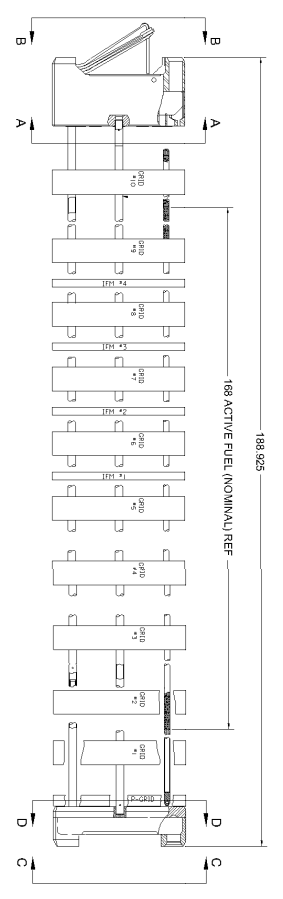
\includegraphics[
  width = 4cm,
  height = 11cm,
  keepaspectratio,
]{AP1000_fuel_assembly.png}
\caption{Schematic of AP1000 fuel assembly with 10 spacer grids and 4 mixing grids.}
\label{fig:ap1000_fuel_assembly}
\end{marginfigure}
\begin{enumerate}
\item Structurally support the fuel pins.  The fuel pins must be restrained against large amplitude vibrations due to the turbulent flow of coolant along the length of the pins.  Vibration, over the long term, results in fuel clad degradation and potential failure.  

\item Enhance convective heat transfer using mixing vanes.  Some of the grid assemblies have vanes that are specifically designed to disrupt the flow field to promote enhanced convective heat transfer along a rod as well as to promote mixing with coolant flowing along adjacent rods.  

\end{enumerate}   
Several of these grids are commonly used both for support and flow mixing.  A schematic of a fuel assembly for the AP1000 is shown in Figure \ref{fig:ap1000_fuel_assembly} with a top view in Figure \ref{fig:ap1000_mv_top_view}.
\begin{marginfigure}
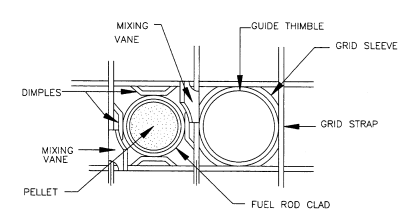
\includegraphics{AP1000_grid_top_view.png}
\caption{Top view of AP1000 grid.}
\label{fig:ap1000_mv_top_view}
\end{marginfigure}


\newthought{Both the grids used} for structural support and those for enhanced flow mixing will result in hydraulic pressure losses that should be taken into account for the engineering analysis of the core.\sidenote{Especially for light water reactors, local pressure conditions in the core can have a big impact on thermal performance.}  The correlations we will use are all designed to provide a reasonable value for a \emph{minor loss coefficient} $(k)$ to capture the hydraulic losses for each spacer or mixing grid.  Generically, pressure drop due to these minor losses are calculated as:
$$\Delta P_{\text{grid}}=k\rho \frac{v^2}{2}$$
or, if USCS units are used:
$$\Delta P_{\text{grid}}=k \rho \frac{v^{2}}{2 g_{c}}$$

\section{De Stordeur Correlation} \index{de Stordeur correlation}
De Stordeur developed a drag coefficient correlation for a variety of wire spacers and spacer grids.\cite{de1961drag} The results are shown in Figure \ref{fig:de_stordeur}.  The pressure drop is calculated from the drag coefficient $C_s$ as shown in Equation \ref{eq:de-stordeur}

\begin{figure}
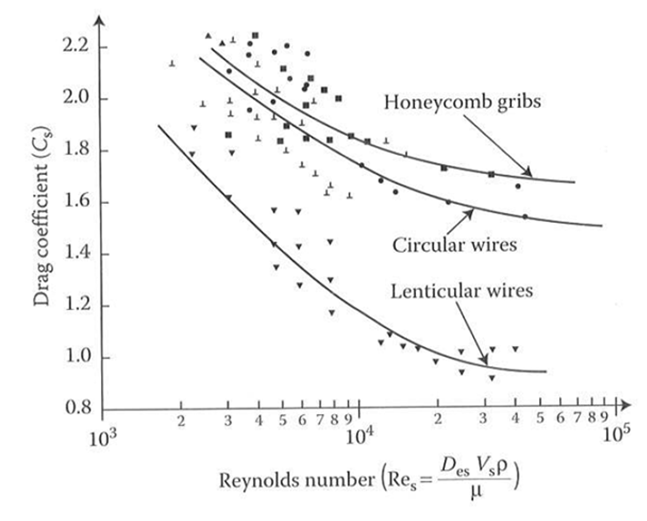
\includegraphics{de_Stordeur.png}
\caption{Drag coefficient results for different spacer wires or mixing grids per de Stordeur.}
\label{fig:de_stordeur}
\end{figure}
\marginnote[-7.5cm]{\textbf{Note: }Take a moment to reflect on the data on which this correlation is based.  Notice the scatter and how the curves provided only approximately capture the general data trends.  Notice how there are more data points at some $\text{Re}_{\text{s}}$ regions and fewer in others. You should keep these observations in mind when you are presenting results of your hydraulic analysis and recognize that precision is limited.}
\marginnote[-2cm]{$\text{Re}_{\text{s}}$ is the Reynolds number in the region of the spacer grid. Note that the characteristic length used, $D_{\text{es}}$, is the \textbf{grid strap thickness} $t$.}

\begin{equation}
\Delta p = C_s\left(\frac{\rho v_s^2}{2} \right)\left(\frac{A_s}{A_v} \right)
\label{eq:de-stordeur}
\end{equation}
where $\rho$ is the fluid density, $v_s$ is the velocity of the coolant \emph{in the spacer region}, $A_v$ is the unrestricted flow area away from the grid or spacer, and $A_s$ is the projected frontal area of the spacer.  Figure \ref{fig:flow_channel_schematic} gives a schematic top-view of a grid spacer.  The projected area of the spacer $(A_s)$ can be calculated as:
\begin{marginfigure}
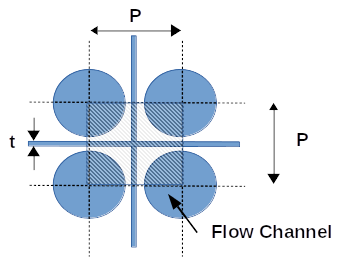
\includegraphics{flow_channel_schematic.png}
\caption{Schematic of flow channel at grid spacer.}
\label{fig:flow_channel_schematic}
\end{marginfigure}
$$A_s = 2Pt - t^2$$
where $P$ is the rod pitch and $t$ is the grid spacer strap thickness.  The flow area in the channel $(A_v)$is given by:
$$A_v = P^2 - \frac{\pi}{4} D^2$$
were $D$ is the fuel rod diameter.  Note that $v_s$ is somewhat \textbf{higher} than the velocity in the channel away from the grid spacer due to the flow constriction at the location of the spacer.  For reactors cooled with incompressible fluids we can estimate $v_s$ as follows:
$$v_s = v \left(\frac{A_v}{A_v - A_s} \right)$$
where $v$ is the fluid velocity in the unobstructed channel.

\newthought{One bothersome detail} is that, for a hydraulic analysis, it would be nice if we could combine the minor losses due to grid spacers with other minor loss coefficients such as core entrance or exit effects.  We want a minor loss coefficent $k$ to use.  Such an expression is given in Equation \ref{eq:k-de-stordeur}.  

\begin{equation}
K_{\text{grid}}^{\text{deStordeur}} = \left(C_s \frac{A_s}{A_{v}} \right)\left(\frac{A_v}{A_v - A_s} \right)^2
\label{eq:k-de-stordeur}
\end{equation} 
Once we calculate $A_v$, $A_s$, and $v_s$, we determine $\text{Re}_{\text{s}}$ and read a value of $C_s$ off the graph, we compute $K_{\text{grid}}^{\text{deStordeur}}$ and find its contribution to pressure drop from $k\rho \frac{v^2}{2}$ like any other component of minor head loss.

\section{Rehme Correlation} \index{Rehme correlation}

A different research group led by Rehme determined, after testing several grid spacers, that the ratio $\sfrac{A_s}{A_v}$ had a more pronounced effect on the pressure drop than indicated by de Stordeur.  They developed a different correlation\cite{rehme1973pressure} of the form given in Equation \ref{eq:rehme-hyd}.

\begin{equation}
\Delta p_{\text{spacer}}=C_v \frac{\rho v^2}{2}\left(\frac{A_s}{A_v} \right)^2
\label{eq:rehme-hyd}
\end{equation} 
Graphs to determine $C_v$ for triangluar and rectangular fuel array spacers are provided in Figure \ref{fig:rehme-tri} and Figure \ref{fig:rehme-square} respectively.\marginnote{\textbf{Note:} $\text{Re}_{\text{B}}$ for this correlation is the Reynolds number in bulk coolant channels.  The characteristic length is the rod diameter $D$.}

\begin{figure}
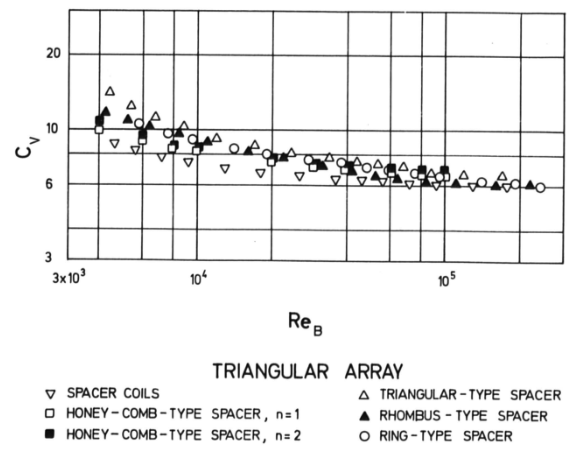
\includegraphics{rehme-tri.png}
\caption{Graph to find $C_v$ for triangular grids.}
\label{fig:rehme-tri}
\end{figure}

\begin{figure}
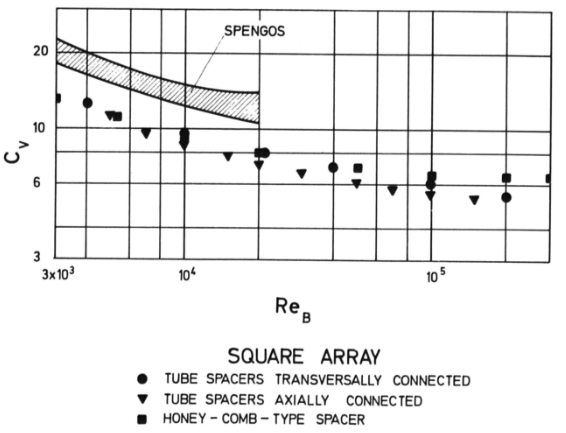
\includegraphics{rehme-square.png}
\caption{Graph to find $C_v$ for rectangular grids.}
\label{fig:rehme-square}
\end{figure}
The area labled ``Spengos'' in Figure \ref{fig:rehme-square} corresponds to the data range in de Stordeur's study.  It should be clear that: a) Rehme created and used data from a wider range of configurations; and b) Rehme will predict a smaller drag coefficient than de Stordeur and thus be expected to preduct a lower $\Delta p$.

\section{In Correlation for PWR Grid Spacers} \index{In's correlation}
A more recently published correlation\cite{in2002empirical} for minor head losses due to grid spacers is due to In and his group.  The equations that comprise the formulation are relatively complex but one compensating benefit is that there is no requirement to read a graph to obtain the coefficient.  This makes use of this correlation particularly ammenable to incorporation into your own hydraulic analysis code.\sidenote{For those so inclined to make such a tool.}  The output is a minor loss coefficient, $K_{\text{grid}}^{\text{In}}$, that you use in a standard minor head loss calculation:
$$\Delta p_{\text{grid}}^{\text{In}} = K_{\text{grid}}^{\text{In}}\frac{\rho v^2}{2}$$
The formula for $K_{\text{grid}}^{\text{In}}$ is given in Equation \ref{eq:k-In}.

\begin{fullwidth}
\begin{multline}
K_{\text{grid}}^{\text{In}} = \underbrace{\left[C_{\text{grid}}^{\text{form}}\frac{\epsilon}{\left(1-\epsilon \right)^2} \right]}_{\text{Term A}} + \underbrace{\left[C_{\text{grid}}^{\text{fric}} \frac{A_{\text{grid,wetted}}}{A_f} \frac{1}{\left(1 - \epsilon \right)^2}\right]}_{\text{Term B}} + \\ \underbrace{\left[C_{\text{rod}}^{\text{fric}} \frac{A_{\text{rods,wetted @ grid}}}{A_f} \frac{1}{\left(1 - \epsilon \right)^2}\right]}_{\text{Term C}}+\underbrace{\left[C_{\text{d,mv}} \frac{\epsilon_{\text{mv}}}{\left(1 - \epsilon_{\text{mv}} \right)^2} \right]}_{\text{Term D}}
\label{eq:k-In}
\end{multline}
\end{fullwidth}
We will discuss each term individually.

\subsection{Term A}
This term tries to capture the effect of form losses for the grid geometry. The coefficient is given by:
$$C_{\text{grid}}^{\text{form}} = 2.75 - 0.27 \log_{10}{(\text{Re})}$$
Where $\text{Re}$ is the Reynolds number evaluated in the flow channel away from the grid.  The parameter $\epsilon$, which is also used in Terms B and C, is really the same as the ratio $\sfrac{A_s}{A_v}$ used in the de Stordeur and Rehme correlations.  It captures the fraction of flow area occluded by the mixing grid.  The nomenclature we will use here is adapted to match the textbook.
$$\epsilon = \frac{A_{\text{grid,frontal}}}{A_f} = \frac{A_s}{A_v}$$
where $A_f$ is just the flow area in the channel away from the grid and the second equality is meant to make the comparison in nomenclature explicit.  

\subsection{Term B} \index{mass flux}
This term tries to capture the pressure losses due to fluid friction with the surface area of the grid strap of height $H$.  For this term we will define the term \emph{mass flux} $(G)$.\marginnote{\textbf{Mass flux (G)} is simply the mass flow rate divided by the cross sectional area: $G = \sfrac{\dot{m}}{A}$.} 

If the strap height, $H \ge \sfrac{3 \times 10^4 \mu_{\text{avg}}}{G_{\text{@ grid}}}$ then:\marginnote[1.0cm]{\textbf{Note: } You should take a few minutes, review the units of dynamic viscosity, $(\mu)$, write down the units of mass flux, $(G)$, and prove to yourself that the ratio of viscosity and mass flux in $\sfrac{3 \times 10^4 \mu_{\text{avg}}}{G_{\text{@ grid}}}$ has units of \underline{length}.}  
The coefficient $C_{\text{grid}}^{\text{fric}}$ is given by:
\begin{multline*}
C_{\text{grid}}^{\text{fric}}=C_{\text{grid,laminar}}^{\text{fric}} \frac{3 \times 10^4 \mu_{\text{avg}}}{G_{\text{@ grid}} H} + \\ C_{\text{grid,turbulent}}^{\text{fric}} \frac{[H - (\sfrac{3 \times 10^4 \mu_{\text{avg}}}{G_{\text{@ grid}}})]}{H}  
\end{multline*} 
Otherwise if $H < \sfrac{3 \times 10^4 \mu_{\text{avg}}}{G_{\text{@ grid}}}$ then: \marginnote[1cm]{\textbf{Note: } The term $G_{\text{@ grid}}$ should be read: ``mass flux at the grid spacer.'' This is different than the mass flux in the rest of the channel around the fuel rod because the grid spacer is obstructing part of the flow area. }
\begin{equation*}
C_{\text{grid}}^{\text{fric}}=C_{\text{grid,laminar}}^{\text{fric}} \frac{3 \times 10^4 \mu_{\text{avg}}}{G_{\text{@ grid}} H}
\end{equation*}
where $C_{\text{grid,laminar}}^{\text{fric}}$ is given by:
$$C_{\text{grid,laminar}}^{\text{fric}}=1.328 \left\{G_{\text{@ grid}} \frac{\left[H - \left(\sfrac{3 \times 10^4 \mu_{\text{avg}}}{G_{\text{@ grid}}}  \right)  \right]}{\mu_{\text{avg}}} \right\}^{-0.5}  $$
and $C_{\text{grid,turbulent}}^{\text{fric}}$ is given by:
$$C_{\text{grid,turbulent}}^{\text{fric}} = 0.523\left\{ \ln{\left[ 0.06 \times G_{\text{@ grid}} \frac{\left[H - \left(\sfrac{3 \times 10^4 \mu_{\text{avg}}}{G_{\text{@ grid}}}  \right)  \right]}{\mu_{\text{avg}}} \right]} \right\}^{-2}  $$

This term also needs $A_{\text{grid,wetted}}$ which, by inspection of Figure \ref{fig:flow_channel_schem2} is given by: $A_{\text{grid,wetted}} = 4(P-t)H.$
\subsection{Term C}\index{McAdams equation}
\begin{marginfigure}
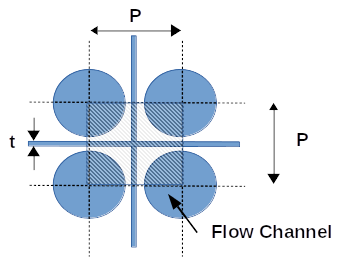
\includegraphics{flow_channel_schematic.png}
\caption{Schematic flow channel in vicinity of spacer grid.}
\label{fig:flow_channel_schem2}
\end{marginfigure}
This term attempts to capture the pressure losses due to fluid friction with the surface are of the fuel rod in the vicinity of the grid spacer.  The formula for $C_{\text{rod}}^{\text{fric}}$ is relatively simple, based on McAdams relation for viscous flow through smooth circular tubes.
$$C_{\text{rod}}^{\text{fric}}=0.184 \text{Re}_{\text{@ grid}}^{-0.2}$$
where $\text{Re}_{\text{@ grid}}$ is the Reynolds number of flow at the grid spacer; $\text{Re}_{\text{@ grid}} = \frac{\rho v_{\text{@ grid}} D_{\text{e, @ grid}}}{\mu}$.  Calculation of the hydraulic diameter requires, in addition to the flow area at the grid spacer, which you already need for this correlation, but also the wetted perimeter. 
$$D_{\text{e, @ grid}} =  \frac{4 A_{\text{flow @ grid}}}{P_{\text{w, @ grid}}} = \frac{4(A_f - A_{\text{grid,frontal}}) }{P_{\text{w, @ grid}}} $$

Recalling a simplified schematic of a flow channel in the vicinity of a spacer grid shown in Figure \ref{fig:flow_channel_schem2}, you should be able to show that the wetted perimeter is: $P_{\text{w, @ grid}}=\pi D + 4(P-t)$.

This term also requires $A_{\text{rod,wetted}}$ which is: $A_{\text{rod,wetted}}=\pi D H$
\subsection{Term D}
\begin{marginfigure}
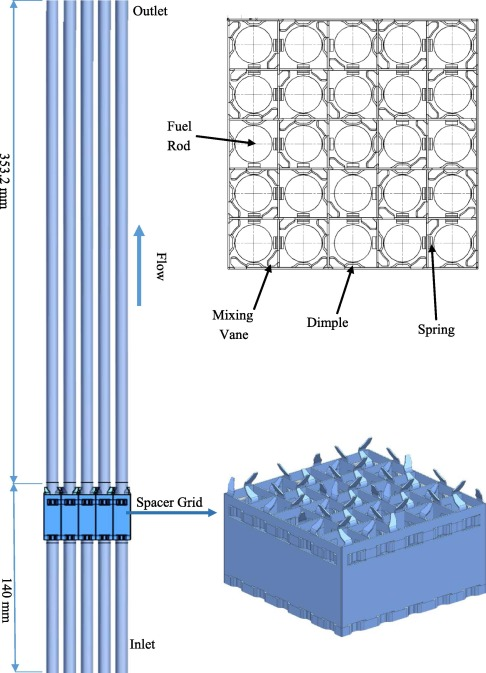
\includegraphics{grid_image.png}
\caption{Grid spacer with mixing vanes.}
\label{fig:grid_image}
\end{marginfigure}
This term attempts to capture the hydraulic effect of any mixing vanes incorported into the grid.  The coefficient $C_{\text{d,mv}}$ is empirically based and expected (by In) to be in the range of 0.6 to 0.8.  They recommend in their paper to use the value: $C_{\text{d,mv}} = 0.72$.  The parameter $\epsilon_{\text{mv}}$ is the ratio of the total ``plugging area'' of the mixing vanes to the bundle flow area away from the grid; it is analagous to the $\epsilon$ used to characterize the extent to which the support grid obstructs the flow channel although there is no reason they should be expected to be the same.  Figure \ref{fig:grid_image} illustrates a spacer grid with mixing vane on the top side.\cite{CHEN20161416}  Note that the mixing vanes necessarily ``obstruct'' the channel more than the spacer grid itself; this is to allow for the vanes to induce vigorous mixing as is desired for improved convective heat transfer performance.

\section{Summary}

Despite the complexity of the In correlation, if you want to incorporate an engineering estimate of minor head losses due to spacers and mixing grids, its use is recommended.  The equations can be (carefully!) encoded using the computing tools of your choice and used without manual reading of graphs.  If a more rigorous analysis is needed, one should commit to detailed computational fluid dynamics and/or experimental studies.

